\chapter[Référence nationale]{\label{I-A}Une référence nationale pour les collections aéronautiques}

\lettrine{L}e \mae du Bourget occupe une position singulière dans le paysage muséographique français. Institution technique aux collections exceptionnelles, il incarne les défis contemporains de la conservation patrimoniale appliquée aux objets technologiques. Son histoire mouvementée témoigne des difficultés rencontrées par les institutions dédiées au patrimoine technique pour trouver leur légitimité, et a façonné un musée unique qui dépasse la simple fonction conservatoire pour s'affirmer comme un acteur central de la recherche aéronautique.

\section{\label{I-A-1}La représentation nationale : un musée aux collections uniques}

\subsection{La lente construction du \mae}

L'histoire du \acf{mae}\footnote{Voir la chronologie de l'histoire du musée en annexe \ref{Ax-A}.} est celle d'un projet persistant, sans cesse reporté et modifié, qui trouve ses racines dès la fin du XIXe siècle dans les aspirations d'associations ou de personnalités liées à l'aéronautique\footcite{terrierAeroportParisBourget2019}. Aujourd'hui encore, il ne cesse d'évoluer : l'année 2025 a ainsi vu, en plus des modernisations logicielles majeures, l'inauguration d'un nouvel espace d'exposition permanente valorisant la tour de contrôle de l'aéroport historique du Bourget\footcite{museedelairetdelespaceHallNavigationAerienne2025}. C'est en effet dans ces locaux que le musée s'est installé en 1973, après une longue période de recherches pour une implantation pérenne. Confronté aux aléas du XXe siècle, aux contraintes de conservation d'objets techniques et aux hésitations ministérielles, le projet d'installation doit sa concrétisation à l'engagement de militaires, de passionnés et au poids de sa mission de vitrine d'un savoir-faire français.

La décision devient effective après la Première Guerre mondiale, premier conflit à exploiter l'importance stratégique de l'aviation. À l'initiative d'Albert Caquot, un conservatoire de l'aéronautique est confié au capitaine Hirschauer : quelques aéronefs trouvent refuge à Issy-les-Moulineaux, avant d'être déplacés à Chalais-Meudon à la suite d'une crue de la Seine. Le musée est officiellement inauguré le 23 novembre 1921 : l'institution naît, mais sans réel ancrage territorial. Pendant l'entre-deux-guerres, d'autres implantations sont tentées, notamment boulevard Victor à Paris. Ces locaux ouverts en 1936 ferment trois ans plus tard à l'aube de la Seconde Guerre mondiale. Bombardements et saisies allemandes interrompent son élan ; à la Libération, le musée réintègre Chalais-Meudon, mais demeure fermé au public durant plus de quinze ans.

S'ensuit une longue période d'incertitudes : entre 1952 et 1972, vingt-et-un sites sont envisagés\footcite{terrierAeroportParisBourget2019}. En 1961, le musée rouvre à Meudon, mais provisoirement. Le « Palais de l'Air » poursuit sa quête de locaux adaptés à la monumentalité de ses collections. En 1973, l'ancien aéroport du Bourget, libéré au profit d'Orly, est retenu comme implantation définitive.

Dès son ouverture, le musée affirme un lien fort avec l’État et l’industrie aéronautique : le prototype Concorde 001 lui est offert par l'état français à l'occasion de son inauguration. Les collections sont progressivement transférées, Chalais-Meudon ferme en 1981, la direction rejoint le Bourget, de nouveaux halls sont ouverts au fil de l’extension du site. C'est avec l'ouverture d'un hall dédié à l'espace en 1983 que le musée prend son nom actuel : \acf{mae}.

Cette consolidation s’accompagne de son intégration à un réseau de musées techniques et de l'armée, et à d'importants chantiers de modernisation : un Planétarium est ouvert en 1985, de nouvelles réserves sont installées à Dugny, l'informatisation des métiers du musée s'amorce dès les années 1990 avec la mise en place de \gls{micromusee} pour les collections, et du \ac{sigb} \gls{alexandrie} pour la bibliothèque. En 2016, l’e-médiathèque est lancée pour gérer les fonds audiovisuels. Cette professionnalisation du musée est notamment marquée en 2002 par sa labellisation \enquote{Musée de France}. Ce mouvement ce poursuit aujourd’hui : les outils de gestion des collections du musées et de la bibliothèque ont été renouvelés définitivement en juillet 2025, de nouveaux espaces de conservation et d’exposition sont en projet, et l'intégration du musée au réseau du Grand Paris Express laisse espérer un surcroît de fréquentation.

Né tout d'abord de ses collections et non d'un site, le \mae, dédié à la mémoire du ciel, est aujourd'hui devenu indissociable de ses locaux emblématiques de l'aéronautique française pour devenir une un musée incontournable.

\subsection{Une institution complexe qui fait référence}

C’est à partir des années 1980 que le musée se structure véritablement, sous l’effet conjoint d’une reconnaissance de l’importance culturelle de l’aéronautique, d’un renouveau muséographique et de son inscription dans les réseaux nationaux. 
Son installation dans les locaux de l'ancien aéroport du Bourget incarne sa double fonction : conservatoire historique de l'aéronautique française, et vitrine stratégique d'un secteur en plein développement. Premier aérodrome civil parisien\footcite{terrierAeroportParisBourget2019}, ce lieu symbolique ancre en effet le musée dans la géographie et l’histoire de l’aviation française. Son lien avec le \ac{siae}, qu’il accueille tous les deux ans, renforce sa fonction de représentation.
La multiplicité des missions du \mae est parfaitement soulignée par Clémence Raynaud dans un article sur les collections iconographiques du \mae : tout d'abord dédié à la documentation de l'histoire et des techniques de l'aéronautique, le musée s'est développé \enquote{comme un établissement à vocation universelle embrassant de multiples aspects du fait aérien, que l’étiquette technique caractérise aujourd’hui d’une manière partielle\footcite{raynaudMuseeTechniqueDhistoire2018}.} Selon l'auteur, qui cite le \ac{psc} 2007, c'est autour des années 2010 que le musée s'affirme comme un \enquote{musée technique, d’histoire et de société}.

C'est là en effet l'un des grands défis auxquels il est confronté : le \mae possède des collections très riches et hétérogènes, sans équivalent national. On y trouve des aéronefs, moteurs, équipements techniques — objets exigeant des conditions de conservation particulières et une expertise rare. Cette spécificité impose des pratiques adaptées et des vocabulaires spécialisés. Mais le musée ne s’y limite pas : maquettes, estampes, objets d’art, uniformes, et, plus récemment, objets civils — vêtements, vaisselle, jouets — reflètent une évolution vers une muséographie anthropologique. Cette inflexion est incarnée notamment par la création d'un département des collections artistiques et anthropologiques, et la diversité des objets conservés se retrouve dans le schéma ci-dessous qui rassemble les différents noms de domaines des collections du musée.

\begin{figure}[htbp]
	\centering
	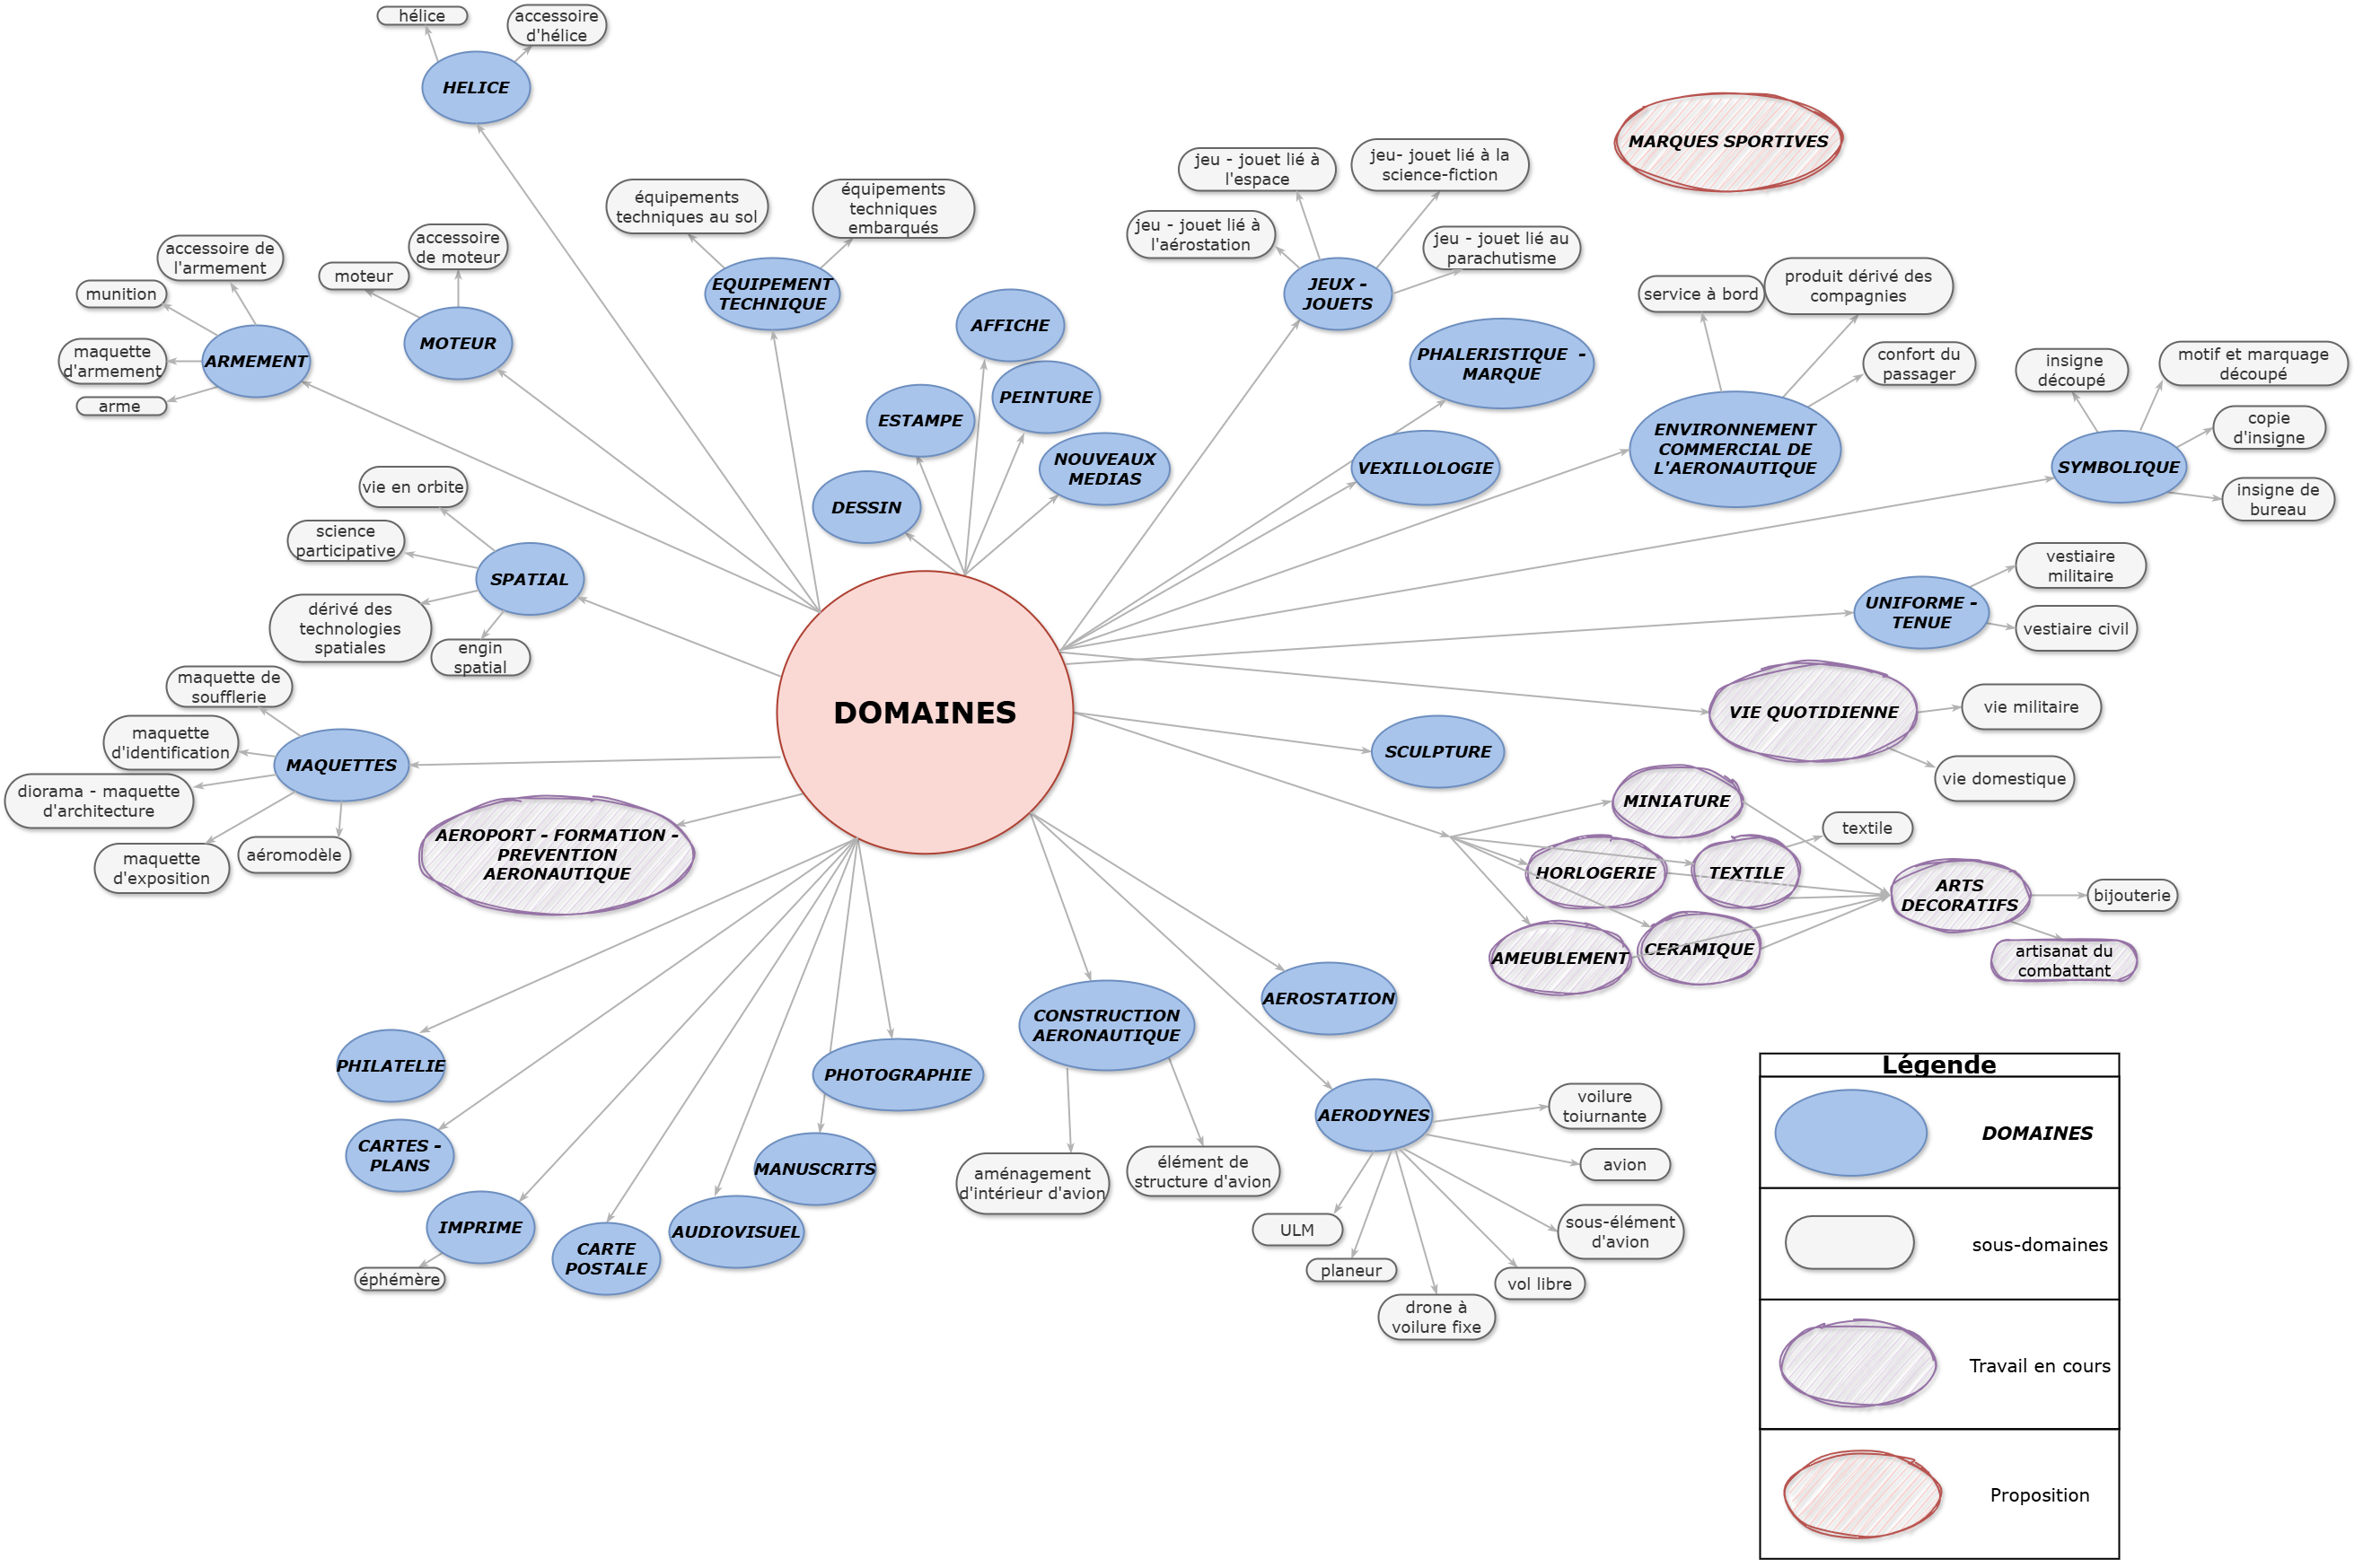
\includegraphics[width=\linewidth]{img/MODEL_domaines.png}
	\caption{Modélisation du thésaurus des domaines utilisés par le \mae}
	\label{fig:model_domaines}
\end{figure}

Le \mae incarne donc des défis propres aux musées techniques, bien différents de ceux des musées de beaux-arts et qui imposent des compétences croisées à la fois techniques et muséales. Les jeunes chargés de collections sont ainsi souvent issus de formations spécialisés — comme les masters du Muséum d’histoire naturelle — et passent par des institutions techniques ou militaires, telles que le musée de la Marine, le musée de l’Armée ou le \ac{cnam}. Ces musées doivent sans cesse composer avec des objets singuliers, souvent massifs, complexes à restaurer et à exposer.

Ces multiples défis sont rappelés par Agnès Mirambet-Paris et François Mirambet : diversité des matériaux, état de dégradation, inadéquation des environnements de conservation, échelle des objets, lourdeur des procédures, et besoin de ressources spécialisées\footcite{mirambet-parisConservationrestaurationPatrimoineTechnique2011}. Ils insistent sur la nécessité du dialogue entre techniciens et restaurateurs :
\begin{quote}
	\og C’est bien par le partage de compétences techniques acquises dans le domaine industriel et celles obtenues dans les écoles de formation à la restauration que pourront se développer pleinement des travaux de restauration\footcite{mirambet-parisConservationrestaurationPatrimoineTechnique2011}.\fg
\end{quote}

Le \mae incarne cette articulation entre expertise technique et exigence muséale. Ses pièces emblématiques — comme le Concorde 001 ou le scaphandre de Jean-Loup Chrétien\footcite{champenoisTresorsMuseeLair} — en font une institution unique, au croisement des enjeux de représentation nationale, de préservation patrimoniale et d’innovation culturelle.


\section{\label{I-A-2}La recherche : le rôle déterminant d'un musée technique}

Le rôle du \ac{mae} ne se cantonne pas seulement à la seule conservation d’objets : celui-ci s'impose en effet comme un acteur essentiel de la recherche au carrefour entre histoire technique, aéronautique, sciences sociales et muséologie.  Le \ac{psc} du \acf{mae}, remanié en 2020, est un précieux témoin du difficile équilibre recherché par le musée pour assurer la visibilité et valorisation de ses fonds auprès du grand public comme de la communauté scientifique.

\subsection{Un acteur central dans les réseaux de recherche aéronautique}

Le \ac{mae} se retrouve en effet, comme bien des musées techniques ou beaux-arts, pris entre différents mondes : musées, bibliothèques, archives, centres de recherches, associations de passionnés... Une grande partie de sa mission consiste donc à assurer la communication entre ces différents qui échangent savoir, pratiques et innovations dans un réseau national comme international.

Ce rôle se manifeste dans la multiplication des expositions temporaires à dimension internationale : l’exposition \emph{Flight}, fruit d’un partenariat avec le Parque de las Ciencias de Grenade, le centre Techmania de Plzeň et l’Institut royal des Sciences naturelles de Belgique, illustre ainsi la capacité du musée à fédérer des acteurs divers autour d’une réflexion sur le vol humain et animal\footnote{Voir \href{https://www.museeairespace.fr/agenda/exposition-flight}{https://www.museeairespace.fr/agenda/exposition-flight}}. De même, des journées d’études, comme celle organisée en 2019 pour le centenaire de l’aviation civile\footnote{Programme disponible sur le site du musée \cite{19192019CentAns}}, réunissent des universitaires, des conservateurs, des ingénieurs ou des amateurs, se retrouvant pour croiser les regards et les méthodes pour améliorer notre compréhension de l'histoire ou encore de la sociologie de l'aéronautique.

L’engagement du musée ne s’arrête pas à la diffusion : il participe à des projets de recherche interdisciplinaires comme le programme C-ADER déposé auprès de l'\ac{anr}, et qui fédère le \ac{c2rmf}, l’Institut de recherche de chimie Paris, l’université de Lorraine et l’Institut de soudure, autour de la  question de la conservation des aéronefs exposés en extérieur\footnote{Voir  \href{https://anr.fr/Projet-ANR-22-CE27-0025}{https://anr.fr/Projet-ANR-22-CE27-0025}}. Ce projet transversal conduira entre autres à l’élaboration d’un thésaurus partagé : celui-ci est une nécessité pragmatique, mais aussi un acte intellectuel qui permet de faire dialoguer chimistes, restaurateurs, conservateurs et historiens avec une même langue. Le musée exerce pleinement dans ce programme son rôle de médiateur et de catalyseur de la recherche.

\subsection{Les outils de la recherche au \ac{mae} : maîtriser la prolifération}

Cette vocation scientifique du \ac{mae} ne saurait prospérer sans une réflexion exigeante sur les outils qui la rendent possible. Le \ac{mae}, à l’instar des grandes institutions patrimoniales, se confronte à un paysage éclaté, où la profusion des bases de données, la diversité des formats et la spécialisation extrême des vocabulaires font facilement obstacle à l’intelligibilité du savoir. C’est pourquoi l’interopérabilité des vocabulaires contrôlés lui est la condition même d’une recherche efficace, capable de relier, d’interroger, de transmettre.

Adopter des normes partagées – \ac{skos}, ISO 25964 – et travailler à l’articulation entre les thésaurus internes et les grands référentiels nationaux comme RAMEAU ou IdRef, c’est inscrire le musée dans une dynamique de réseau : permettre à ses données de circuler, de s’enrichir, d’être réutilisées, c’est-à-dire de vivre\footcite{hudonISO25964Pour2012a,chichereau_normes_2007,nouvel_thesaurus_2019}. Ce chantier, encore inachevé, appelle la mobilisation de toutes les compétences, la prise en compte des spécificités du vocabulaire aéronautique et la volonté de ne jamais sacrifier la précision technique à la seule facilité d’alignement. Il s’agit moins de proclamer une normalisation absolue que d’élaborer des passerelles, des zones de contact intelligentes où la diversité des pratiques s’ordonne sans se dissoudre.

L’autre versant de cette politique documentaire concerne la gestion des archives numériques liées aux œuvres. La numérisation systématique des ressources iconographiques, la production croissante de dossiers de collection et de documentation, loin de n’être qu’un progrès matériel, font peser sur l’institution une responsabilité nouvelle : garantir la pérennité, l’intégrité, la traçabilité de ces flux d’information\footcite{ministere_de_la_culture_documenter_2020,bechard_archives_2020}. S’accumuler n’est pas conserver : le musée doit s’astreindre à élaborer des procédures d’archivage conformes aux référentiels nationaux\footcite{comite_interministeriel_aux_archives_de_france_referentiel_nodate}, à choisir des solutions logicielles adaptées (GED, SAE), à former son personnel à la rigueur de la gestion documentaire.

Cette maîtrise n’est pas un luxe mais une exigence : elle fonde la valeur scientifique des collections, assure leur transmissibilité, et garantit au musée sa capacité à irriguer, au-delà de ses murs, la réflexion sur le patrimoine aéronautique. Ainsi, le \ac{mae}, loin de se contenter d’accumuler des objets ou des fichiers, s’impose par la cohérence de ses choix et l’exemplarité de ses pratiques comme une référence nationale et un acteur majeur de la recherche.



\bigskip
\bigskip
\bigskip

Cette multiplicité d'acteurs et d'exigences pose un défi documentaire majeur : comment organiser l'information pour qu'elle soit simultanément accessible aux spécialistes de l'aéronautique, aux historiens, aux conservateurs et au grand public ? La question dépasse la simple indexation : elle interroge la conception même des vocabulaires contrôlés dans un contexte muséal technique. Les thésaurus traditionnels, conçus pour des domaines disciplinaires homogènes, peuvent-ils répondre aux besoins d'une institution qui articule technique, histoire, patrimoine et médiation culturelle ?

Cette problématique se complique encore du fait du statut particulier du \mae au sein du \minarm, qui impose des contraintes supplémentaires d'harmonisation avec les systèmes documentaires militaires.